\chapter{Геймификация бега}
Для геймификации бега была придумана концепция интерактивного сюжета, в рамках которой игрок оказывается в некой ситуации, разворачивающейся по мере прохождения точек интереса на карте. Также по мере развития сюжета игроку предлагаются некоторые препятствия, которые он должен физически обойти.
\section{Интерактивный сценарий}
Интерактивный сценарий представляет из себя иерархическую структуру данных со следующими объектами:
\begin{figure}[H]
	\centering
	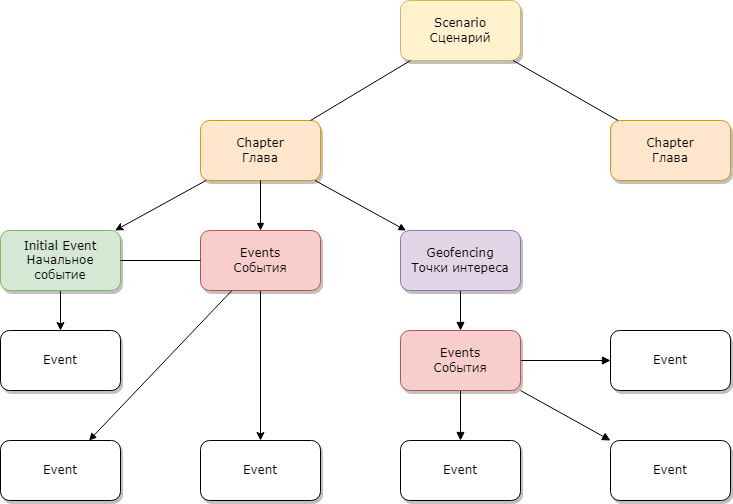
\includegraphics[width=\textwidth]{flesh/runGamification/scenario.png}
	\caption{\label{fig:scenario_components}Схема компонентов сценария}
\end{figure}
\section{Система виртуальных препятствий}
Виртуальное препятствие является концептом, которого не существует в реальном мире, но он генерируется игрой и заставляет игрока выполнить какое-либо действие, связанное с бегом. Сейчас мы различаем следующие виды препятствий:
\begin{description}
	\item[Дикие собаки] Данное препятствие имитирует бег за игроком диких собак, которые могут нанести ему вред : для преодоления препятствия необходимо ускориться за опредлённое время.
	\item[Сильный ветер] Данное препятствие имитирует сильный ветер, сносящий игрока. Для преодоления препятствия необходимо ``подыграть'' игре и снизить скорость за определённое время.
\end{description}
\subsection*{Генерация препятствия}
Бла бла
\subsection*{Валидация препятствия}
Бла бла
\section{Система точек интереса}
Бла бла
\subsection*{Генерация точки интереса}
Бла бла
\subsection*{Действия, выполняемые при попадании в точку интереса}
Бла бла